\documentclass[tikz,border=2mm]{standalone}
\usepackage{tikz}
\usetikzlibrary{patterns}
\usepackage{amssymb}
\usepackage{amsmath}
\tikzstyle{stuff_nofill}=[rectangle,draw,font={}]
\tikzstyle{stuff_fill}=[rectangle,draw,fill=white,minimum size=1.4em,label={center:}]

\begin{document}
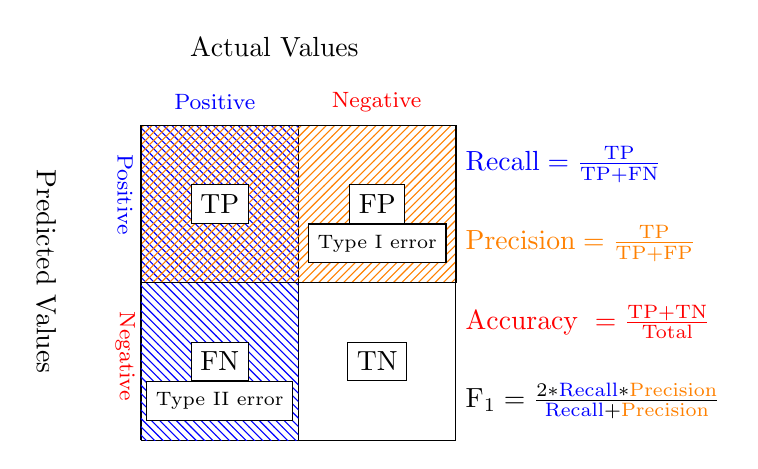
\begin{tikzpicture}
\node[right] at (0.5,5.0) {Actual Values};
\node[right] at (0.3,4.3) {\footnotesize \textcolor{blue}{Positive}};
\node[right] at (2.3,4.3) {\footnotesize \textcolor{red}{Negative}};
\node[label=below:\rotatebox{-90}{ Predicted Values}] at (-1.2,3.8) {};
\node[label=below:\rotatebox{-90}{ \footnotesize \textcolor{blue}{Positive}}] at (-0.2,4) {};
\node[label=below:\rotatebox{-90}{ \footnotesize \textcolor{red}{Negative}}] at (-0.2,2) {};
\draw[step=2.0,black,thin] (0,0) grid (4,4);
\fill[pattern=north west lines, pattern color=blue] (0,0) rectangle (2,4);
\draw[pattern=north east lines, pattern color=orange] (0,2) rectangle (4,4);
\node at (1,3)[stuff_fill] {TP};\node at (1,1)[stuff_fill] {FN};
\node at (3,3)[stuff_fill] {FP};\node at (3,1)[stuff_fill] {TN};
\node at (3,2.5)[stuff_fill] {\scriptsize Type I error};\node at (1,0.5)[stuff_fill] {\scriptsize Type II error};
\node at (4,3.5)[right,color=blue]{$\text{Recall}=\frac{\text{TP}}{\text{TP+FN}}$};
\node at (4,2.5)[right,color=orange]{$\text{Precision}=\frac{\text{TP}}{\text{TP+FP}}$};
\node at (4,1.5)[right,color=red]{$\text{Accuracy }=\frac{\text{TP+TN}}{\text{Total}}$};
\node at (4,0.5)[right]{$\text{F}_1=\frac{2*\text{\textcolor{blue}{Recall}}*\text{\textcolor{orange}{Precision}}}{\text{\textcolor{blue}{Recall}+\textcolor{orange}{Precision}}}$};

\end{tikzpicture}

\end{document}